\documentclass[UTF8, a4paper, linespread=1.5]{article}

\usepackage{tcolorbox, listings, algorithm, minted, algpseudocode}
\usepackage{geometry, savesym, amsmath, enumerate, indentfirst, color, amsthm, bm, extarrows, ulem}
\usepackage{amssymb}
\usepackage{nameref, hyperref}
 \geometry{top=3cm, bottom=3cm, left=1.5cm, right=1.5cm}

\usepackage{enumitem}
\setenumerate[1]{itemsep=0pt,partopsep=0pt,parsep=\parskip,topsep=5pt}
\setitemize[1]{itemsep=0pt,partopsep=0pt,parsep=\parskip,topsep=5pt}

\renewcommand\contentsname{Contents}

\tcbuselibrary{skins, breakable, theorems}

% \setlength{\leftskip}{10pt}
\setlength{\parindent}{10pt}
% \setlength{\parskip}{2em}
\renewcommand{\baselinestretch}{1.3}

\newcounter{RomanNumber}
\newcommand{\mrm}[1]{(\setcounter{RomanNumber}{#1}\Roman{RomanNumber})}

\newtcbtheorem{thm}{}
  {enhanced, theorem name and number, code={\edef\@currentlabelname{#2}}, 
  frame code={
        % \path[thick, draw] (frame.north west) -| (frame.north east) -| (frame.south east) -| (frame.south west) -| (frame.north west);
        \path[thick, draw] (frame.north west)  +(.5\baselineskip,0) -| +(0,-.5\baselineskip);
        % \path[thick, draw] (frame.north east) +(-.5\baselineskip,0) -| +(0,-.5\baselineskip);
        % \path[thick, draw] (frame.south west) +(.5\baselineskip,0) -| +(0,.5\baselineskip);
        \path[thick, draw] (frame.south east) +(-.5\baselineskip,0) -| +(0,.5\baselineskip);
    },
    left=1mm, right=1mm, top=1mm, bottom=1mm,
    colback=black!5,
    colframe=red!75!black,
    colbacktitle=black!0,
    coltitle=black!100,
    fonttitle=\bfseries}{thm}


\usepackage{environ}
\RenewEnviron{math}{%
\begin{align*}
\BODY
\end{align*}
}

\title{CS217 -- Algorithm Design and Analysis \\ Homework 5}
\date{\today}
\author{Not Strong Enough}



\begin{document}

    \begin{thm}{}{}
        For a graph $G = (V, E)$, let $\tau(G)$ denote the size of a minimum vertex cover, and $\nu(G)$ the size of a maximum matching. Recall the two linear programs VCLP and MLP. Let $\tau_f(G) := {\rm opt}({\rm VCLP}(G))$ and $\nu_f(G) := {\rm opt}({\rm MLP}(G))$. Note that
        $$
        \nu(G) \leq \nu_f(G) = \tau_f(G) \leq \tau(G),
        $$
        where the equality in the middle follows from Strong LP Duality. Also, if $G$ is bipartite, then the equality holds throughout in (1). Let us say a graph $G$ is {\it VCLP exact} if $\tau(G) = \tau_f(G)$, and {\it MLP exact} if $\nu(G) = \nu_f(G)$. As we already know, a bipartite grpah $G$ is both VCLP exact and MLP exact.
        
        From now on, suppose that $G$ is {\it not} bipartite but $\tau(G) = \tau_f(G)$.
        
        \begin{enumerate}
            \item Give an example of such a graph $G$ that is not bipartite but still VCLP exact.
            \item Give an example of a graph $G$ that is MLP exact but not VCLP exact.
            \item Suppose $G$ is VCLP exact. Let $Y \subseteq V(G)$ be a minimum vertex cover. Let $\mathbf{x}$ be an optimal solution of MLP($G$). Show that $x_e = 0$ if $e \subseteq Y$ (i.e., if both endpoints of $e$ are in the cover).
            \item Show that such a graph $G$ has a matching of size $|Y|$, and thus is MLP exact, too.
        \end{enumerate}
    \end{thm}

    \begin{center}
        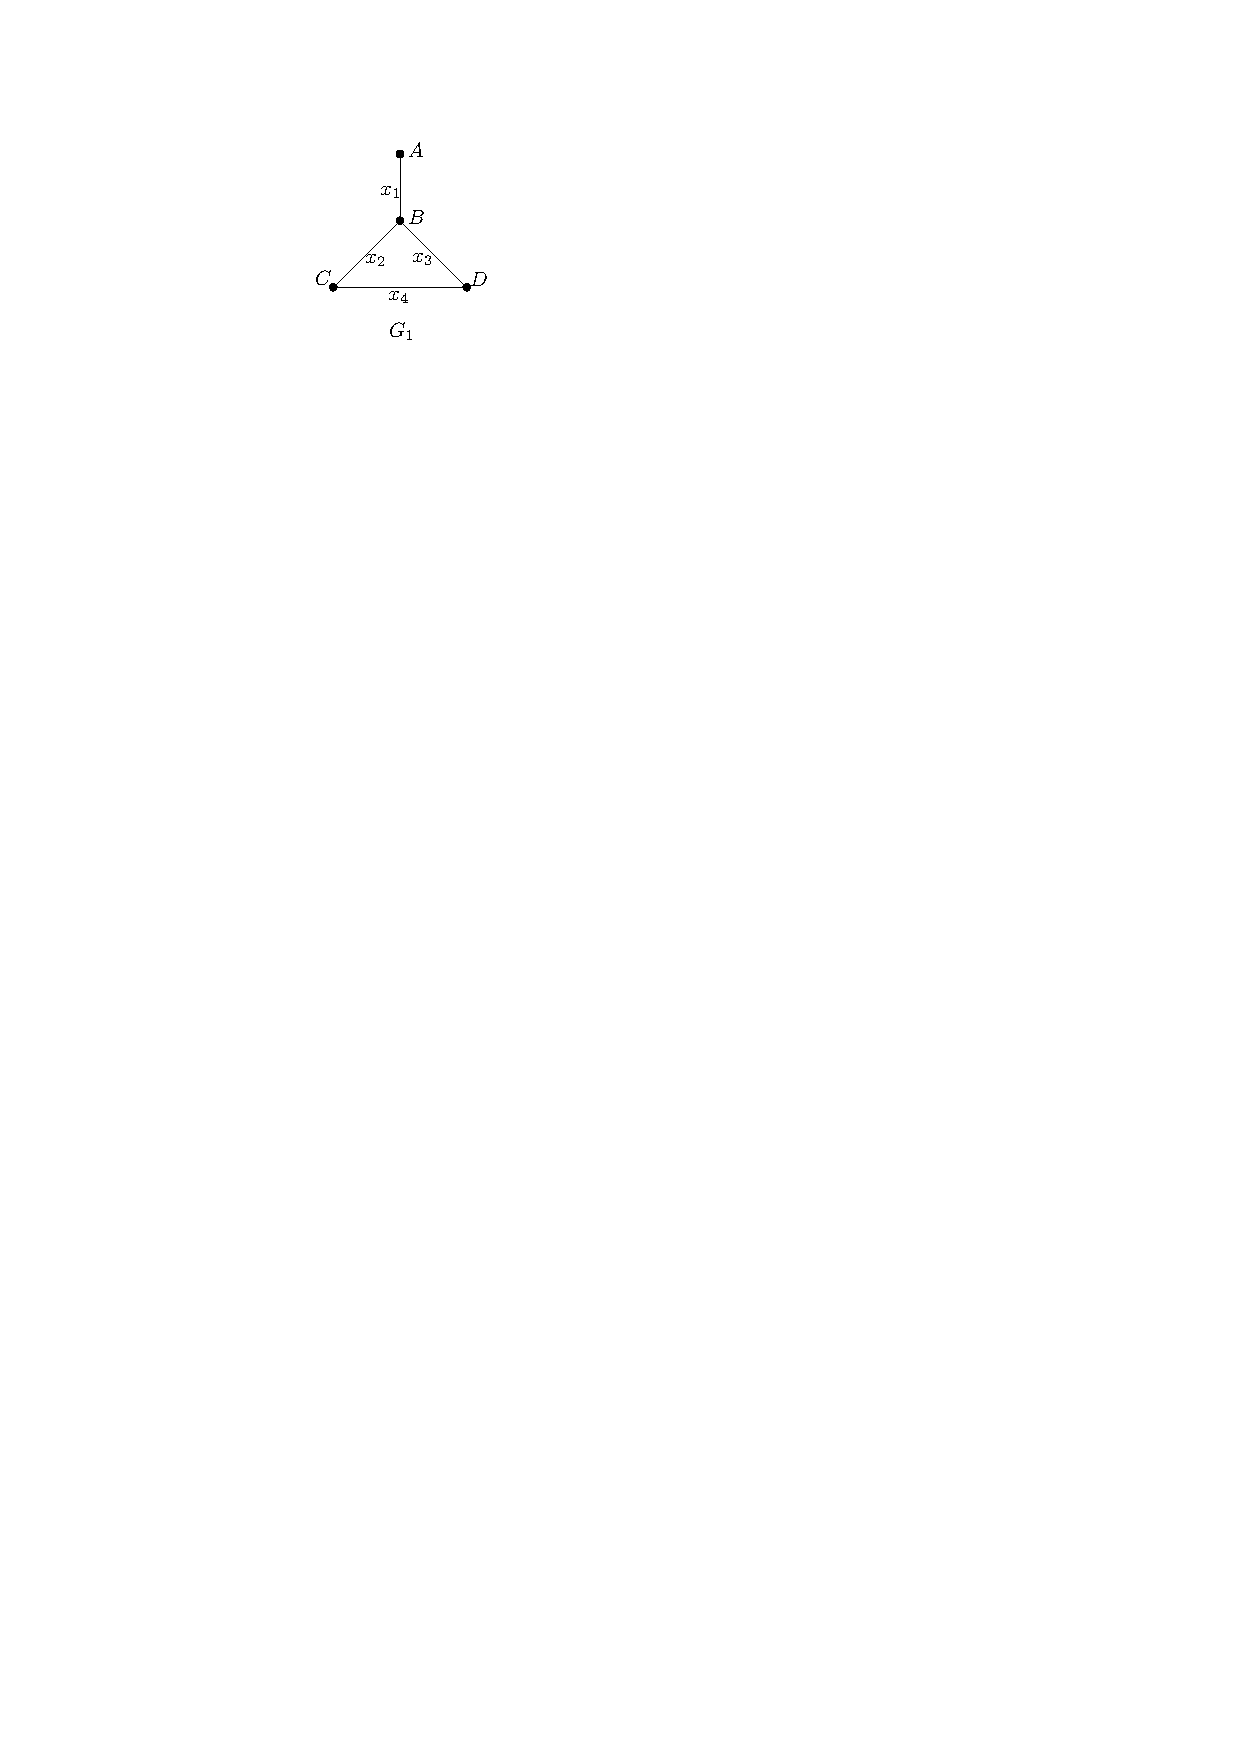
\includegraphics[width=0.16\textwidth]{figure4_1.pdf}
        \hspace{3cm}
        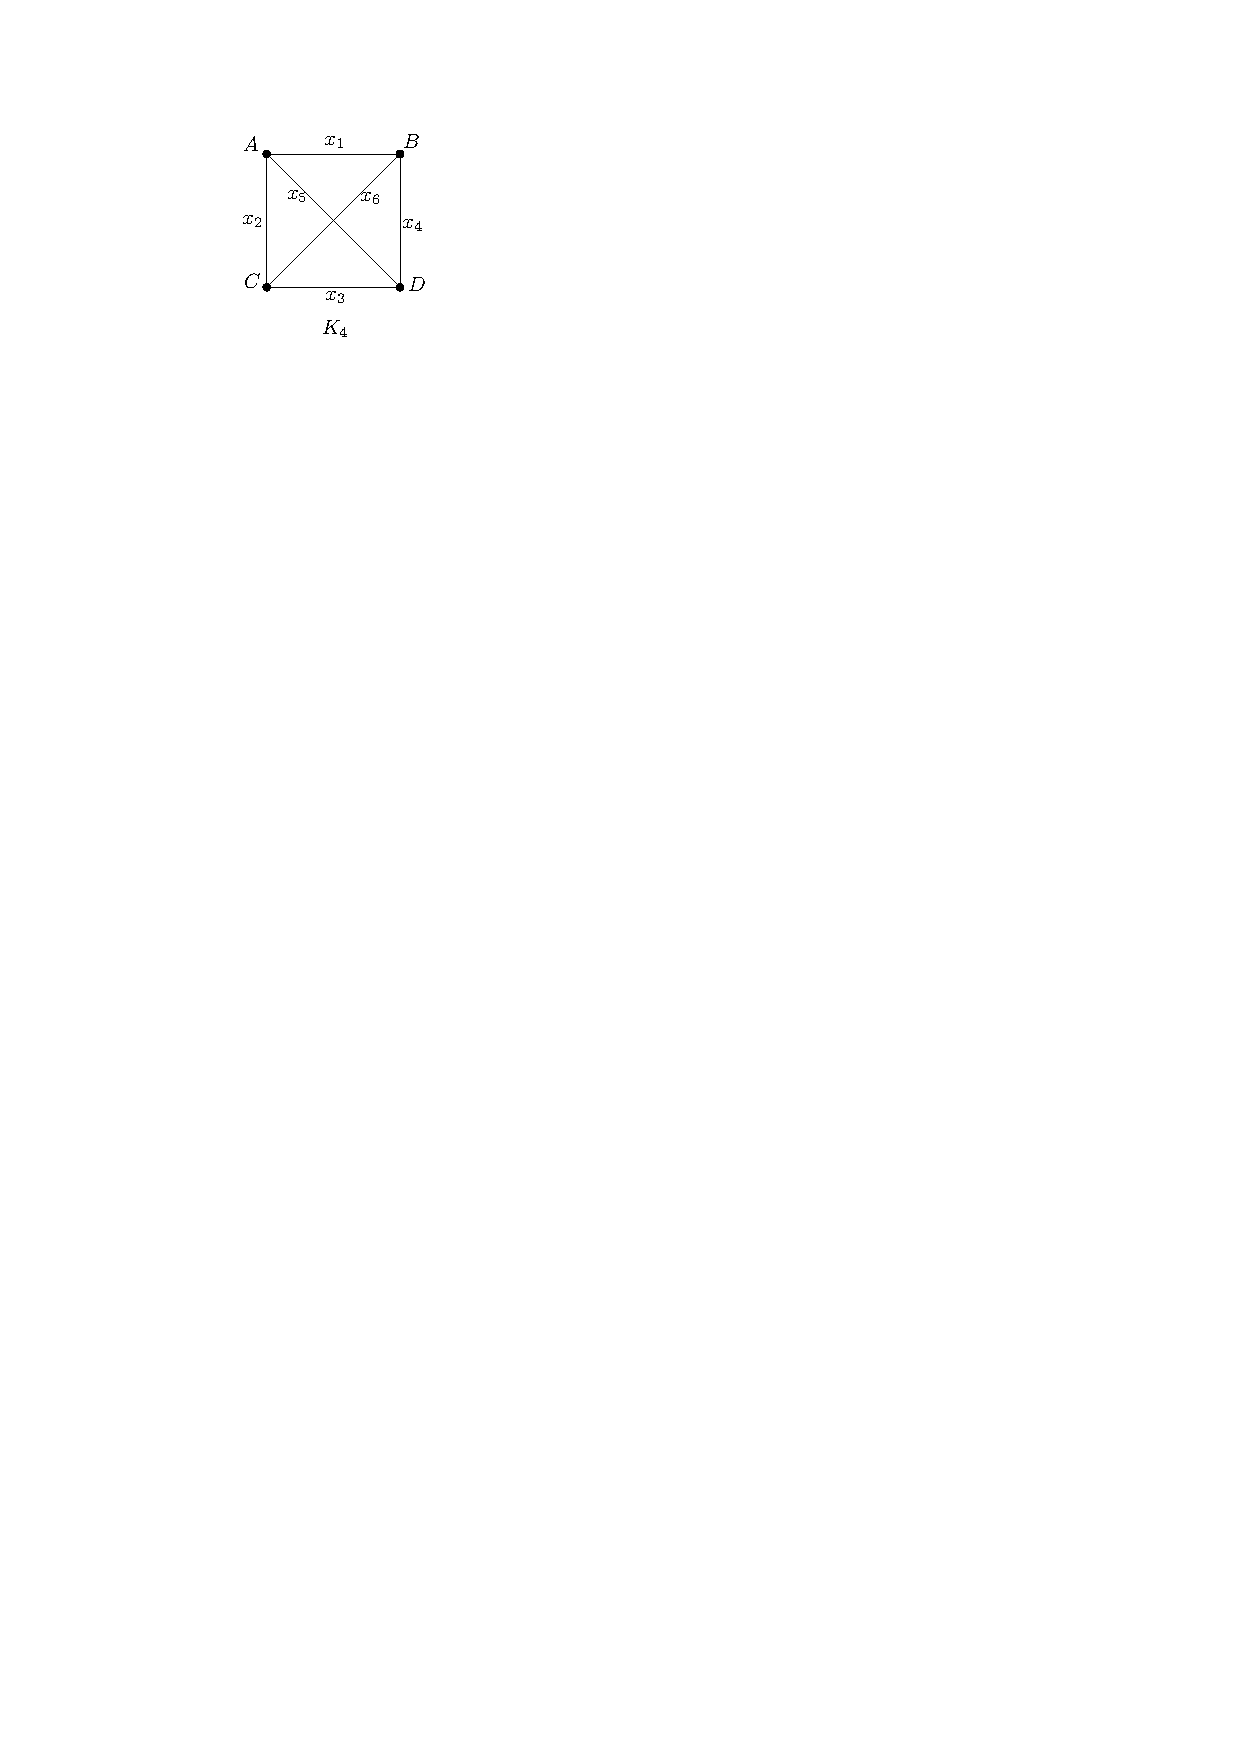
\includegraphics[width=0.16\textwidth]{figure4_2.pdf}
    \end{center}

    \begin{proof}[Solution.]
        \begin{enumerate}
            \item The example is $G_1$ in the upper left. It is not bipartite since $B, C, D$ constitute an odd cycle.
            
            The minimum vertex cover of $G_1$ can be $\{B, C\}$ or $\{B, D\}$, with size $2$. So $\tau(G_1) = 2$.
            
            VCLP$(G_1)$ is
            \begin{center}
                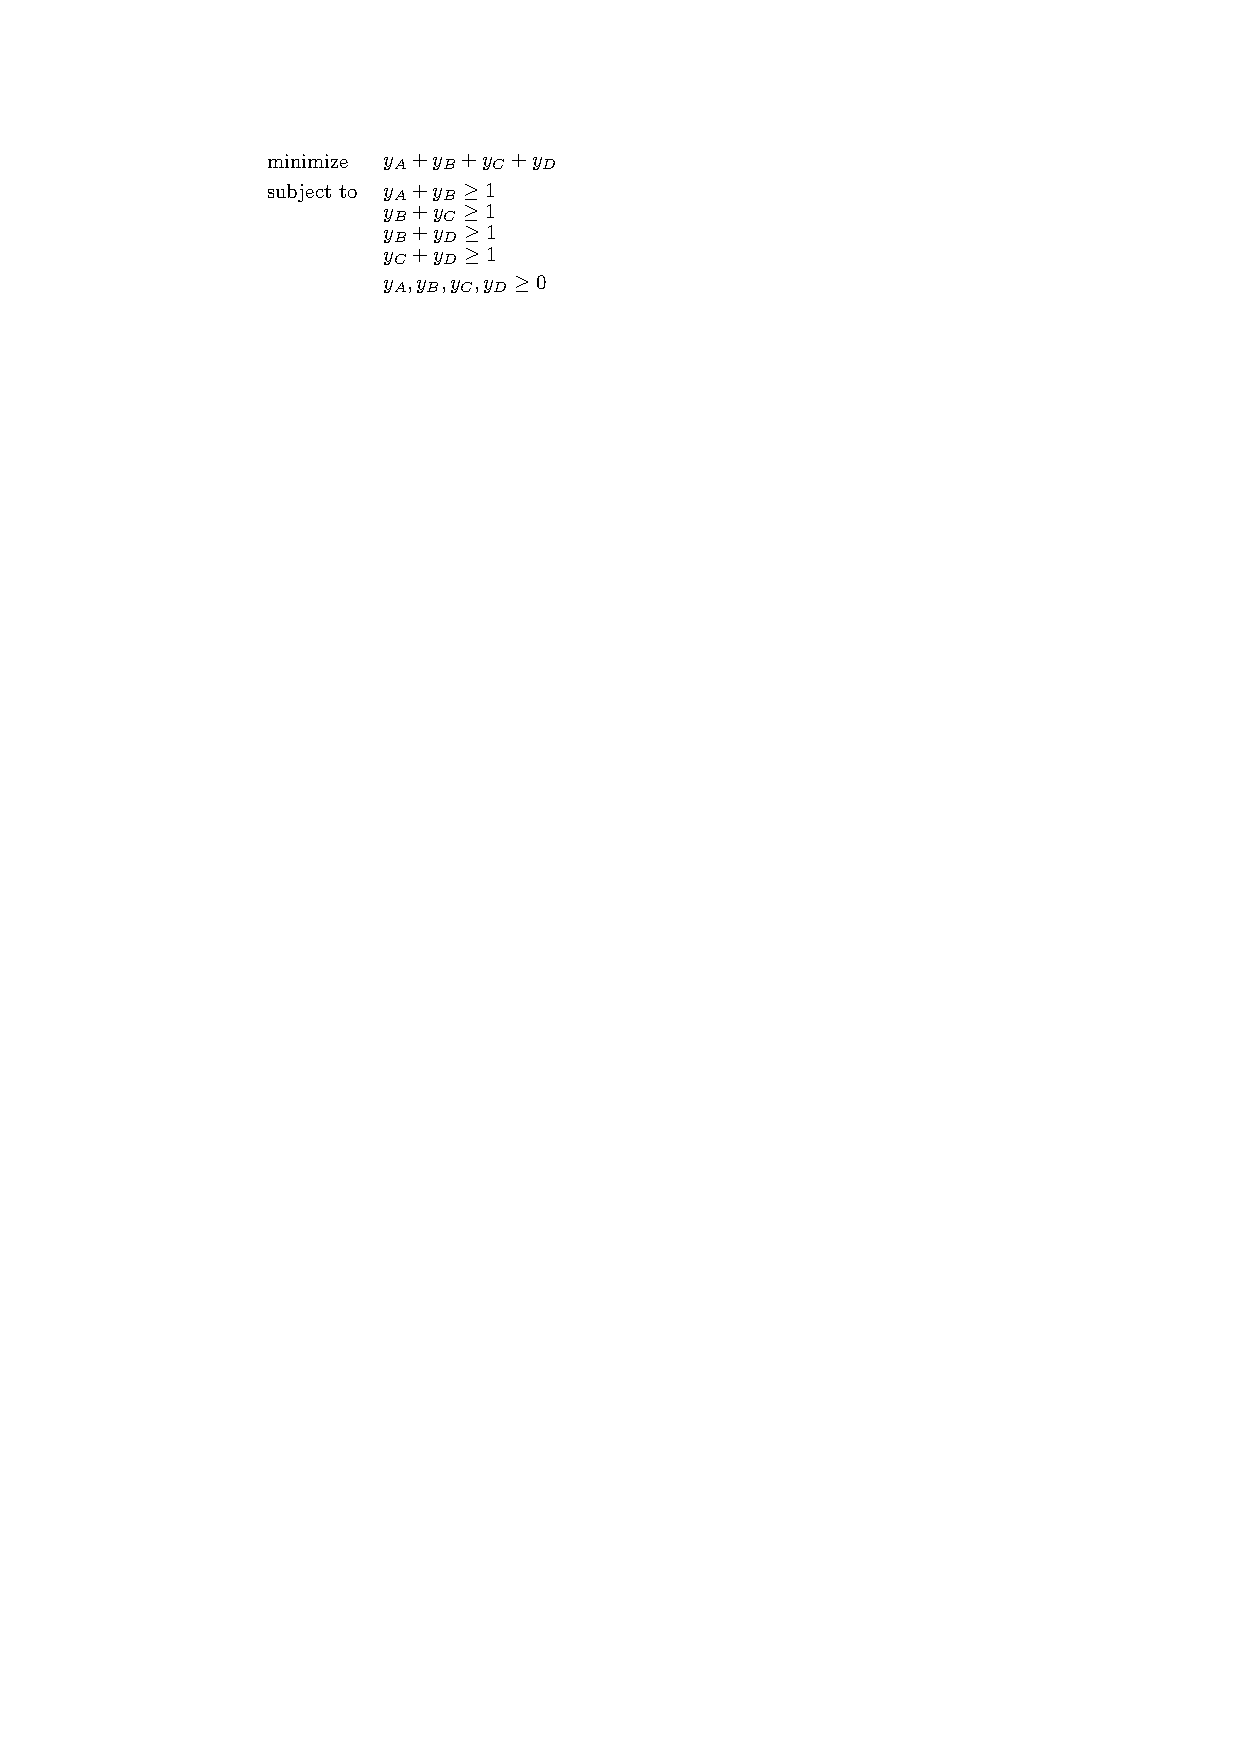
\includegraphics[width=0.28\textwidth]{VCLP4_1.pdf}
            \end{center}
            Note that if we add up the constraints $y_A + y_B \geq 1$ and $y_C + y_D \geq 1$, we get $y_A + y_B + y_C + y_D \geq 2$, which gives a lower bound of the target function.
            
            Since $\tau(G_1) = 2$, it follows that the lower bound is tight. Hence $\tau_f(G_1) = \tau(G_1) = 2$.
            
            So $G_1$ is an example which is not bipartite but still VCLP exact.
            
            \item The example is $K_4$ in the upper right. The minimum vertex cover can be $\{A, B, C\}, \{A, B, D\}, \{A, C, D\}$ and $\{B, C, D\}$, with size $3$. So $\tau(K_4) = 3$.
            
            However, by setting the value of each vertex to $0.5$, we find that all edges are exactly covered ($y_u + y_v = 1$ for edge $(u, v)$). So $\tau_f(K_4) \leq 2$, and thus $K_4$ is not VCLP exact.
            
            Now consider the maximum matching and MLP. Obviously we can only match $2$ pairs of vertices. So $\nu(K_4) = 2$, and $\nu_f(K_4) \geq 2$ follows. Since we already know that $\tau_f(K_4) \leq 2$ and $\nu_f(K_4) = \tau_f(K_4)$ by Strong LP Duality, we can conclude that $\nu(K_4) = \nu_f(K_4) = \tau_f(K_4) = 2$. Therefore $K_4$ is MLP exact.
            
            So $K_4$ is an example which is MLP exact but not VCLP exact.
        \end{enumerate}
    \end{proof}


\end{document}

